% Collective Intelligence 2014 LaTeX format
% Adapted from ACM Large format by Walter S. Lasecki
%
%
% Steps to compile: latex, bibtex, latex, latex
%
\documentclass[prodmode,acmtap]{ci2016}

% Metadata Information
\acmVolume{2}
\acmNumber{3}
\acmArticle{1}
\articleSeq{1}
\acmYear{2010}
\acmMonth{5}

% Package to generate and customize Algorithm as per ACM style
\usepackage[ruled]{algorithm2e}
\SetAlFnt{\algofont}
\SetAlCapFnt{\algofont}
\SetAlCapNameFnt{\algofont}
\SetAlCapHSkip{0pt}
\IncMargin{-\parindent}
\renewcommand{\algorithmcfname}{ALGORITHM}

% Page heads
\markboth{T. Maillart}{On the Importance of Co-Located Meetings for Community Building and Long-Term Online Production}

% Title portion
\title{On the Importance of Co-Located Events for Community Building and Long-Term Online Production}
\author{THOMAS MAILLART \affil{UC Berkeley}}
% NOTE! Affiliations placed here should be for the institution where the
%       BULK of the research was done. If the author has gone to a new
%       institution, before publication, the (above) affiliation should NOT be changed.
%       The authors 'current' address may be given in the "Author's addresses:" block (below).
%       So for example, Mr. Fogarty, the bulk of the research was done at UIUC, and he is
%       currently affiliated with NASA.


% At a minimum you need to supply the author names, year and a title.
% IMPORTANT:
% Full first names whenever they are known, surname last, followed by a period.
% In the case of two authors, 'and' is placed between them.
% In the case of three or more authors, the serial comma is used, that is, all author names
% except the last one but including the penultimate author's name are followed by a comma,
% and then 'and' is placed before the final author's name.
% If only first and middle initials are known, then each initial
% is followed by a period and they are separated by a space.
% The remaining information (journal title, volume, article number, date, etc.) is 'auto-generated'.



\begin{document}


\maketitle
\noindent Nearly all online communities organize co-located meetings, such as conferences, un-conferences, and hackathons. These events are short, fast-paced, yet they are intended to enable social interactions and fast-circulation of informal knowledge between attendants. There is however a dearth of knowledge on the contribution of co-located events to community enhancement and long-term online production. Here, I study a community of astrophysicists involved in open and reproducible data science. Over the span of data collected (4 years), five co-located meetings were organized. Each meeting triggered contrasted immediate effects regarding collaboration, but all of them had significant long-term enhancing effects on community building and online knowledge production. These results illustrate how punctual co-located meetings change the way contributors engage with their community once they have resumed their routine work online. 

% Head 1
\section{Introduction}
Early on, organization science researchers have pointed out the importance of special \emph{``kairos"} moments, with their own purpose and genuine timing, by opposition to \emph{``kronos"} routine moments \cite{orlikowski2002s}. 
%{\bf [say a bit more here, especially about the long-term effects of special moments]}. 
The development of online collaboration tools has created a striking contrast between these moments: routine work is mostly performed online, whereas co-located meetings address completely different problems, ranging from prototyping and showcasing \cite{trainer2014community} to strengthening social ties \cite{ducheneaut2005socialization}, teaching tools and on-boarding newcomers \cite{von2003community}, deliberating on an agenda for future work, as well as for solving community governance issues \cite{o2007emergence}. On the contrary, routine work consists mostly in a stream of prioritized issues with some degree of required collective coordination to solve them \cite{dabbish2012social}. Thus, co-located events are less about immediate knowledge production than about organizing online collective production on the long-term, once community members have gone back home, sometimes all over the country or the world. Co-located events are characterized by numerous and fast-paced social interactions or pair-programming, involving small-talk as well as rapid exchange of knowledge between tens if not hundreds of people over short periods of time, usually ranging from one day to a week. \\

\noindent Although direct observation, quantification and modeling of subtle inter-personal interactions during physical is usually complicated \cite{choudhury2002sociometer,pentland2005human,onnela2014using}, co-located events trigger cascades of contributions with long-term memory, which allow measuring their after-effects on community and building and follow-up online production.  Furthermore, co-located meetings, and hackathons in particular, may be associated with super-linear productive bursts, which stem from \emph{critical, self-sustained, cascades of contributions} among developers \cite{sornette2014much}, with similitudes with super-linear laws of productivity (e.g., number of patents) and interactions (e.g., phone calls) in cities \cite{bettencourt2007growth,schlapfer2014scaling}.\\

\noindent Here, I study how co-located meetings generate cascades of contributions. These cascades may be of two kinds: Either they occur on a personal project (i.e., code repository), or they are contributed on a shared project. While the former contribution cascades reflect single-minded concentration on a problem, the latter cascades display the intention and capacity to interact with others. Both cascade types co-exist, but the amount of contribution cascades initialized on shared code repositories is a signature of a community having built social ties, and vividly sharing problems and solutions, during or following co-located events.

\section{Data and Method}
\noindent The present study is carried on for the American Astronomical Society (AAS) HackDays (2013, 2014 and 2015) and Astro Hack Weeks (2014 and 2015). The former events are intended to \emph{``write code or work on some other project, fast, [and] fully execute it in one day"} and the latter events correspond to a \emph{``week-long summer school, hack week, un-conference focused on astrostatistics and data-intensive astronomy"}.\footnote{Astro Hack Day, \url{http://www.astrobetter.com/wiki/AAS_HackDay_2014}; and Astro Hack Week, \url{http://astrohackweek.github.io}} The activity (i.e., both number of contributors and projects contributed to) and production (i.e., code and issue submissions) per time unit have been queried from the GitHub Archive.\footnote{GitHub Archive, \url{https://www.githubarchive.org/}.} And community members considered here are selected for their participations to at least one Astro Hack Week.\\

\noindent Considering the aforementioned co-located hackathons, I first compare the number of contribution cascades initiated on {\it personal} and {\it shared} code repositories, and how they have evolved over the period of scrutiny (from January 1st, 2012 until December 31st, 2015). I then show that contribution cascades are heavy-tailed (with a significant difference between personal and shared contributions). I finally provide insights on the overall flow of contributions by the community, again with a distinction between personal and shared contributions.
 
\section{Results}
The community of astrophysicists involved in open and reproducible data science \cite{fernandoperezblog} has been active for four years at least. Since January 1st, 2012, five co-located meetings were organized to shape a community (64 members in this study), and to build collectively programming and data handling tools to modernize their practice of astrophysics.\\

\noindent Each hackathon had its own impact on the community as measured by the number of contribution cascades initiated on personal and shared code repositories (resp. $c_i$  and $c_s$; see Figure \ref{cascade_inits}A). The first  AAS HackDay {\bf (a)} had limited immediate measurable impact but contributed to increase the baseline of $c_i$ and $c_s$ over the next year, while the following hackathons had a significant immediate impact on contribution cascade initializations, followed by a slow decay until the next co-located meeting. The decays are best fitted by power laws $\sim t^{-\alpha}$ with $\alpha \approx 0.7(1)$ for {\bf (c)}, {\bf (d)} and {\bf (e)} (both for personal and shared contribution cascades), which is reminiscent of critical cascades in social media \cite{crane2008}.\\

\begin{figure}[h]
\centering
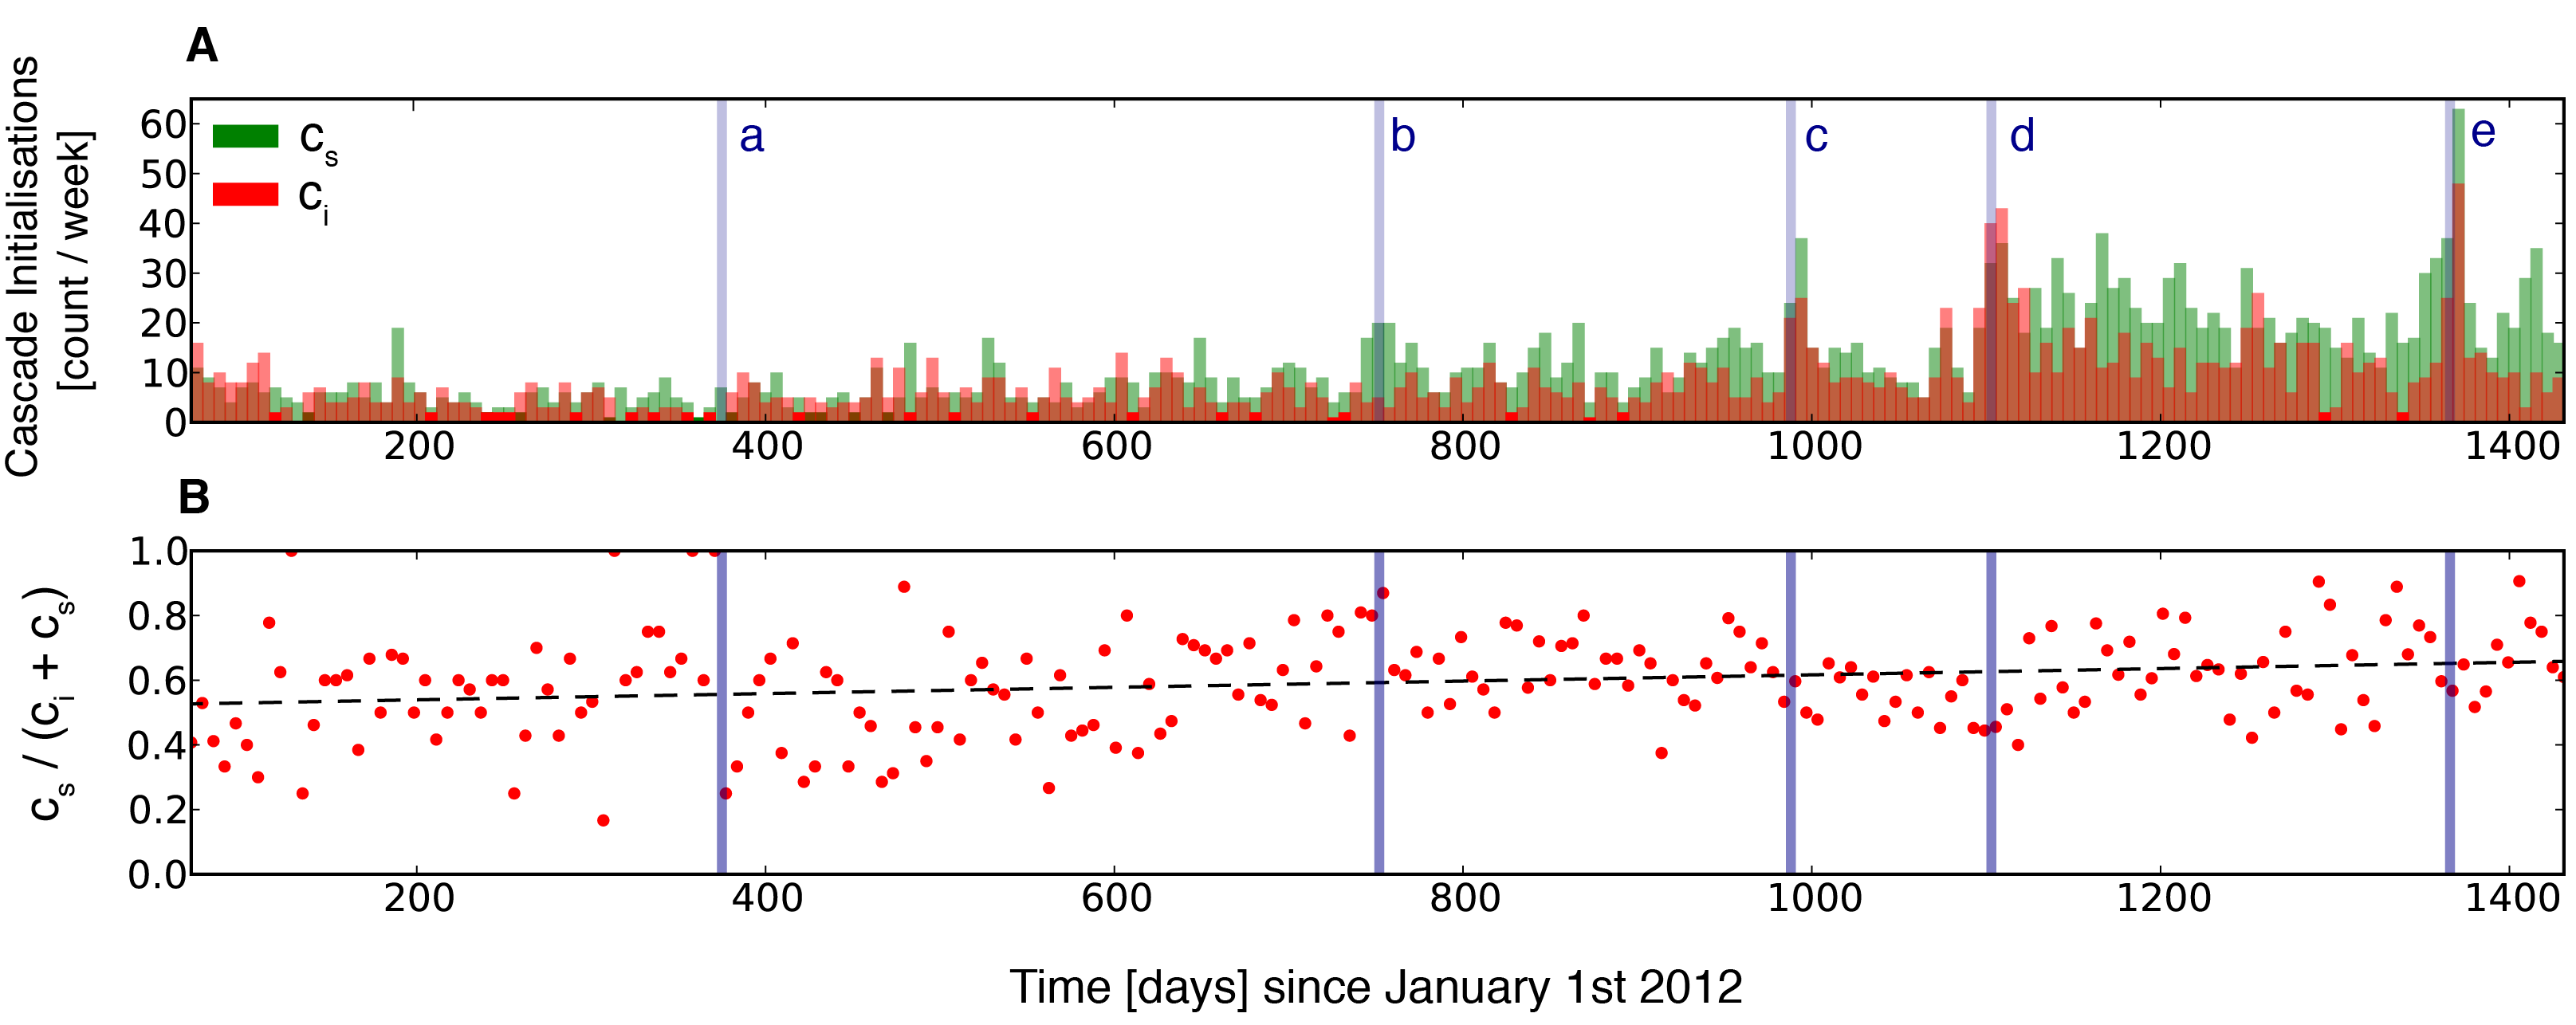
\includegraphics[width=16.5cm]{individual_vs_interactive_cascades.png}
\caption{{\bf A.} Progression of individual vs. collective contribution cascade initializations (resp. $c_i$ and $c_s$), punctuated by 5 hackathons: {\bf (a)} HackDay 2013, {\bf (b)} HackDay 2014, {\bf (c)} Astro Hack Week 2014, {\bf (d)} HackDay 2015, and {\bf (e)} Astro Hack Week 2015. {\bf B.} The share of collective contribution cascades initiated $c_s$ over all cascade initializations ($c_i + c_s$) increases linearly (3.5\%/year; $p < 0.001$; dashed line). It is important to note that $r = c_s / (c_i + c_s) > 0.5$ on average. As time passes, each hackathon triggers a larger impulse on cascade initializations.}
\label{cascade_inits}
\end{figure}

\noindent The ratio  $r = c_s /(c_i + c_s)$ of contribution cascade initializations in shared repositories $c_s$ over all cascade initializations increased linearly (3.5\% per year; $p < 0.001$)  and from $r_0 \approx 0.5$ in 2012 (see Figure \ref{cascade_inits}B). The contribution of each hackathon to $r$ is however contrasted: HackDays 2014 and 2015 (resp. {\bf b} and {\bf d}) had a long-standing impact, while Astro Hack Week 2014 {\bf (c)} had rather a negative immediate impact on $r$ and the situation for Astro Hack Week 2015 {\bf (e)} remains unclear.\\

\noindent While contribution cascade initializations illustrate the intention to work individually or to share improvements, the number of contributions (i.e., the actual cascade size) after initialization helps quantify the long-term commitment to  respectively individual or collective projects. The distributions of contribution cascades to {\it individual} and {\it shared} projects are respectively log-normal and power law (not represented). On average contribution cascades to individual projects are longer ($ \mu_{i} = 29.60$) compared to contributions to shared projects ($ \mu_{s} = 16.33$). However, the former are less skewed ($ \gamma_{i} = 8.02$) compared to the latter ($\gamma_{s} = 31.54$) with maximum number of contributions being respectively $1,348$ and $5,415$. In other words, contribution cascades to shared projects in the community of astrophysicists are much more extreme. This reflects the difficulty to organize collective work (compared to own work), but when it is established, collective work is likely to be considerably more productive.

%\begin{table}[h]
%\begin{center}
%    \begin{tabular}{lccccc}
%    Cascade Type       & median & mean  & std. deviation & skewness & maximum \\ \hline
%    Individual project & 7.00   & 29.60 & 88.00          & 8.02     & 1,348    \\
%    Shared project     & 2.00   & 16.33 & 127.69         & 31.54    & 5,415    \\
%    \end{tabular}
%\end{center}
% %\caption{}
%\label{cascade_sizes}
%\end{table}

\section{Conclusion}
Co-located meetings are special moments of importance for community enhancement and long-term online production. Here, I have investigated how five hackathons have fostered online collaboration in a community of astrophysicists. I find that the four most recent hackathons have triggered productive bursts of contribution both to shared and individual projects. Their relative contributions to collective work cascades initializations are however contrasted. Finally, long-term online production is embodied by the size of contribution cascades: contribution cascades to shared projects in the community of astrophysicists are much more extreme, reflecting the difficulty to organize collective work, and at the same time, its amazing productivity when collective work cascades are unlocked.

\clearpage

% Bibliography
\bibliographystyle{ci-format}
\bibliography{../bib/astrohackweek.bib}


\end{document}
